%%%%%%%%%%%%%%%%%%%%%%%%%%%%%%%%%%%%%%%%%%%%%%%%%%%%%%%%%%%%%%%%%%%%%%%%
\chapter{Introduction}
\label{chapter:introduction}
%%%%%%%%%%%%%%%%%%%%%%%%%%%%%%%%%%%%%%%%%%%%%%%%%%%%%%%%%%%%%%%%%%%%%%%%
\localtableofcontents

%%%%%%%%%%%%%%%%%%%%%%%%%%%%%%%%%%%%%%%%%%%%%%%%%%%%%%%%%%%%%%%%%%%%%%%%%%%%%%%
\section{Context \& Motivation}
\label{section:ch1-context_and_motivation}
%%%%%%%%%%%%%%%%%%%%%%%%%%%%%%%%%%%%%%%%%%%%%%%%%%%%%%%%%%%%%%%%%%%%%%%%%%%%%%%

%%%%%%%%%%%%%%%%%%%%%%%%%%%%%%%%%%%%%%%%%%%%%%%%%%%%%%%%%%%%%%%%%%%%%%%%%%%%%%%
\subsection{Context}
\label{subsection:ch1-context}
%%%%%%%%%%%%%%%%%%%%%%%%%%%%%%%%%%%%%%%%%%%%%%%%%%%%%%%%%%%%%%%%%%%%%%%%%%%%%%%

With the surge in data collection and computing resources over the last 20 years, the interest and use cases for Machine Learning have grown exponentially.
More specifically, Deep Learning, a subfield of Machine Learning, consisting of training Deep Neural Networks on high-level
data (images, sounds, texts) have shown great achievements.
In recent years, Deep Neural Networks achieve state-of-the-art performances in a variety of domains such as image recognition~\cite{lecun1998gradient,krizhevsky2012imagenet,he2016deep,tan2019efficientnet}, object detection~\cite{redmon2016you,liu2016ssd,redmon2017yolo9000}, natural language processing~\cite{merity2016pointer,radford2018Language,brown2020language}, speech recognition~\cite{hinton2012deep,abdel2014convolutional,yu2016automatic}, etc.

\begin{figure}[t]
  \centering
  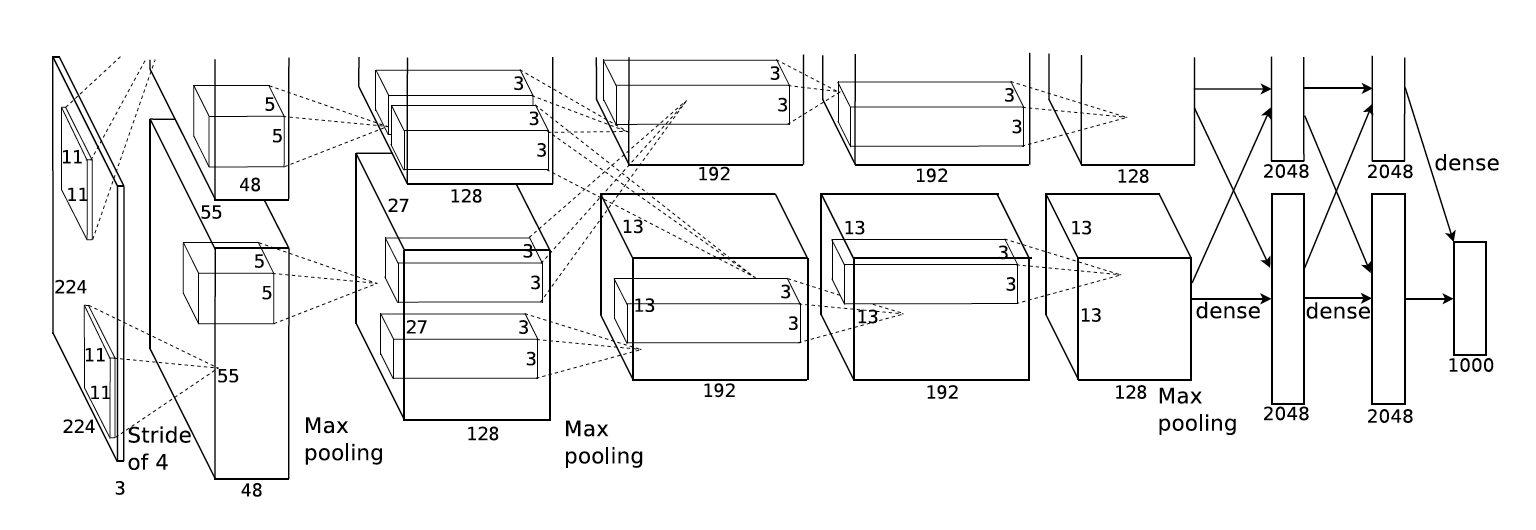
\includegraphics[scale=0.2]{figures/chapter1/alexnet.png}
  \caption{This figure shows the neural network architecture (AlexNet) proposed by~\citet{krizhevsky2012imagenet} which won the ImageNet Large-Scale Visual Recognition Challenge in 2012.}
  \label{figure:ch1-alexnet_network}
\end{figure}

One of the first breakthroughs of Deep Learning was during the 2012 ImageNet Large-Scale Visual Recognition Challenge~\cite{ILSVRC15} which consists of evaluating algorithms for object detection and image classification.
In this challenge, \citet{krizhevsky2012imagenet} achieved \nth{1} place and beat every other participants by a 10.8\% margin with a neural network architecture called \emph{AlexNet} (see Figure~\ref{figure:ch1-alexnet_network}). 
The main reasons for such performance are three fold: first, they used a network architecture with more than 60 million parameters which was significant for the computational resources of the time; they used the ImageNet database~\cite{deng2009imagenet} which consists of 1.2 million labeled images with 1000 different classes for training their network; finally, they used graphics processing units (GPUs) to speed up the mathematical operations, reducing training time from several months to just a few days. 

\begin{table}[t]
  \centering
    {\small
    \begin{tabular}{llcc}
      \textbf{Computer Vision Models} & & & \\
      \toprule
      Authors & Models & \#Params & TOP-5 Acc. \\
      \midrule
      \citet{krizhevsky2012imagenet} & AlexNet~ & 61M & 84.7\% \\
      \citet{simonyan2014very} & VGG & 144M & 92.0\% \\
      \citet{he2016deep} & ResNet-152 & 60M & 93.8\% \\
      \citet{szegedy2017inception} & Inception-ResNet-v2 & 56M & 95.1\% \\
      \citet{xie2017aggregated} & ResNeXt-101 & 84M & 95.6\% \\
      \citet{hu2018squeeze} & SENet & 146M & 96.2\% \\
      \citet{huang2019gpipe} & GPipe & 556M & 97.0\% \\
      \bottomrule \\
      \textbf{Natural Language Processing Models} & & & \\
      \toprule
      Authors & Models & \#Params & Score \\
      \midrule
      \citet{peters2018deep} & ELMo & 94M & xxx \\
      \citet{radford2018improving} & GPT & 110M & xxx \\
      \citet{devlin2019bert} & BERT & 340M & xxx \\
      \citet{radford2019language} & GPT-2 & 1.5B & xxx \\
      \citet{shoeybi2019megatron} & MegatronLM & 8.3B & xxx \\
      \citet{rosset2020turingnlg} & T-NLG & 17B & xxx \\
      \citet{brown2020language} & GPT-3 & 175B & xxx \\
      \bottomrule
    \end{tabular}
    }
    \caption{The first table shows different networks trained for computer vision with their number of parameters and accuracy that came up in the years after AlexNet. This second table shows different networks trained for Natural Language Processing tasks that came out in the last three years.}
  \label{table:ch1-networks_parameters}
\end{table}

Since this result, many different architectures came out, with more and more parameters leading some years later to near perfect accuracy on the ImageNet Dataset and Computer Vision task in general.
Table~\ref{table:ch1-networks_parameters} shows the different architectures that came out in the years after AlexNet.
While most new architectures have been proposed based on intuition and test and learn approaches, recent research \cite{tan2019efficientnet,rosenfeld2020a} have examined the relationship between the number of parameters (model size), the size of the dataset and the accuracy.
For computer vision models, \citet{tan2019efficientnet} have shown that the relation between model size and accuracy seems to obey a power law. 
This discovery leads them to propose an efficient neural network with similar or higher accuracy than existing ones.  
% In computer vision, \citet{tan2019efficientnet} have shown that this relationship seems to obey a power law leading them to propose an efficient neural network with similar or higher accuracy.
For Natural Language Processing (NLP) neural networks, this relationship has also been observed and given the availability of large-scale datasets (Common Crawl dataset~\cite{raffel2019exploring} constitutes nearly a trillion words), researchers have been able to scale their models culminating in the 175 billion parameters GPT-3 model proposed by~\citet{brown2020language}. 

As a result, higher performing models in computer vision and natural language processing have enabled the deployment and use of these models in real-world applications such as autonomous vehicles~\cite{fagnant2015preparing}, translation~\cite{wu2016google}, vocal assistants~\cite{li2017acoustic}.
Translation and voice assistants are now used by millions of people around the world and the autonomous vehicles could reshape the transportation industry over the next decade.





% Since large scale neural networks have the ability to \emph{memorize} their training data and demonstrate generalization abilities \cite{zhang2016understanding}, building models with hundreds of millions or even billions of parameters leads naturally to an increase in the accuracy of the task at hand.
% This simple fact is certainly the reason for the race of bigger and bigger models.


% Although, it has been known for quite some time \cite{} that scaling dataset size 
%
% EfficientNets[TL19] also appear to obey an approximate power-law relation between accuracy and model size. 
%
% => power-law scalings between performance and dataset size. 
% [BB01] Scaling to very very large corpora for natural language disambiguation
% \cite{banko2001scaling}
% [Goo01] A Bit of Progress in Language Modeling
% \cite{goodman2001bit}
%
% \cite{banko2001scaling,goodman2001bit}
%
% => caling between model size and data size; their work is perhaps the closest to ours in the literature
% [HNA+17] Deep learning scaling is predictable, empirically
% \cite{hestness2017deep}
% [HAD19] Beyond human-level accuracy: Computational challenges in deep learning
% \cite{hestness2019beyond}
%
% Very recent work [RRBS19b] studies scaling with both dataset size and model size for a variety of datasets, and fits an
% ansatz similar to ours.
% \cite{rosenfeld2020a}

%%%%%%%%%%%%%%%%%%%%%%%%%%%%%%%%%%%%%%%%%%%%%%%%%%%%%%%%%%%%%%%%%%%%%%%%%%%%%%%
\subsection{Motivation}
\label{subsection:ch1-motivation}
%%%%%%%%%%%%%%%%%%%%%%%%%%%%%%%%%%%%%%%%%%%%%%%%%%%%%%%%%%%%%%%%%%%%%%%%%%%%%%%

% Pourquoi j'ai fait cette thèse

% -> consomation energétique,
% -> robustesse aux attaques
% -> complexité, analyse.


In recent years, researchers have searched for networks with higher and higher accuracy in order to build models that can be deployed into real-world applications. 
However, recent finding suggests that the accuracy cannot be the only metric to optimize. 
Neural networks, when implemented in a critical decision process, need to be efficient, secure and interpretable.
Although accurate, large neural networks lack these properties.

\paragraph{Efficient Neural Networks}
With the growing concern over data privacy, methods such as \emph{federated learning} are gaining ground.
Federated learning involves training a model across multiple decentralized devices (\eg, smartphones) with local data sample. 
This avoids the step of centralizing all users' data into one server, thus addressing the issue of data privacy.  
In this setting, the training needs to be performed with limited computational and memory resources. 
More generally, building efficient neural networks can have upside.
Indeed training state-of-the-art models on the ImageNet dataset needs gigabytes of memory and can take several days to train on a single GPU. 
NLP models are even worst, for example, it has been estimated that the GPT-3 model with 175 billion parameters requires 355 years of training on a single GPU and \$4,600,000 to train on a cloud-based compute platform~\cite{li2020overview}.
Thus, building efficient neural networks can reduce training time, cost and allow for faster research and development.


\begin{figure}[htb]
  \centering
  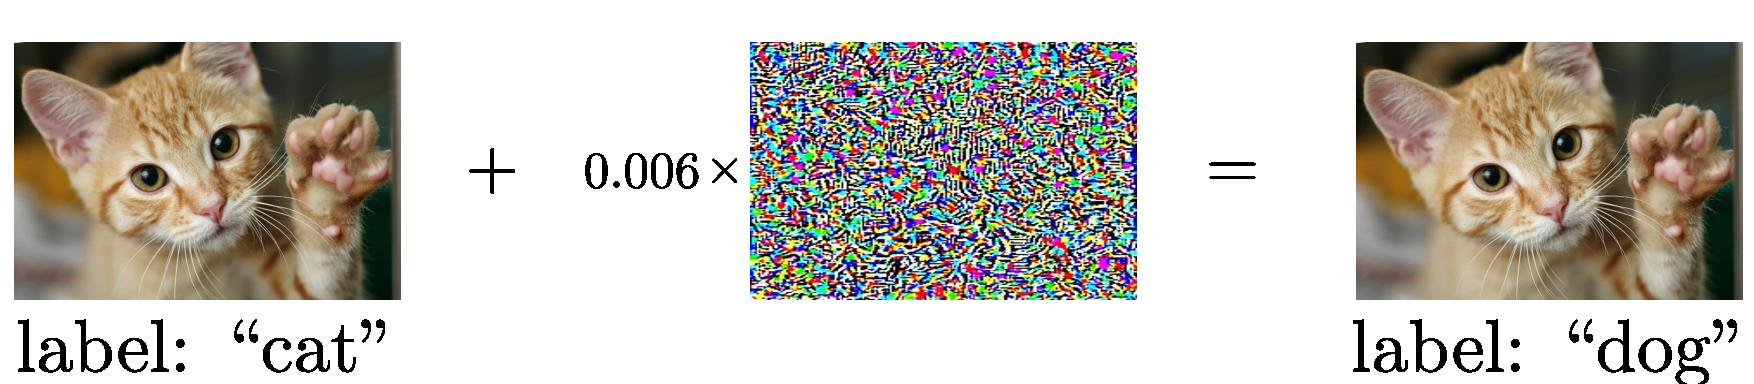
\includegraphics[width=\textwidth]{figures/chapter1/ExampleAdversarialCatDog.pdf}
  \caption{Example of Adversarial Attack on an image. The small perturbation (center) is added to the original image (left) leading to an adversarial image (right).}
  \label{figure:adversarial_image_example}
\end{figure}

\paragraph{Secure and Interpretable Neural Networks}
% Some specific use cases can tolerate a few mistakes by an automatic system.
% Autonomous vehicle aren't one of it.
A mistake by the neural network governing the drive of an autonomous vehicle can lead to injuries or even death, hence a model with perfect accuracy is required.
However, it is difficult to guarantee that no errors will be made.
% Having the possibility to interpret and to understand the error made is important to correct it.
Having the ability to interpret and understand the error is therefore essential to prevent its recurrence.
Very large neural networks with millions, or more, parameters act as a kind of black box and are difficult to interpret.
% Recently, \citet{lundberg2017unified} proposed an algorithm to interpret the decision of machine learning models,   
Algorithms \cite{lundberg2017unified} for interpreting the decision of a machine learning models scale exponentially with the number of parameters making it impractical for large neural networks. 
% interpretation for machine learning models scale exponentially with the number of parameters making it impractical for large neural networks.
Furthermore, large neural networks due to a high complexity and expressivity exhibit instability to small perturbations of their inputs.
The best example of this phenomenon is the vulnerability of neural networks to \emph{adversarial examples}, \ie, imperceptible variations of the natural examples, crafted to deliberately mislead the models~\cite{globerson2006nightmare,biggio2013evasion,szegedy2013intriguing} (see Figure~\ref{figure:adversarial_image_example}). 
This behavior can cause serious security problems for neural networks used for critical decision-making for example self-driving cars.



% The neural network governing the decision of an autonomous vehicle has to be accurate. A high accuracy will guarante 
%
% The accuracy the neural network of an autonomous vehicle govern the way it will drive and therefore its safety.
% But when a wrong decision happens which could lead to injury of even death, affected parties will want to review and interpret the decision.
% Large neural network have been known to act as a kind of black box  


% First, large neural networks are computationally expensive and not energy efficient.
% The training of a sate-of-the-art models on the ImageNet dataset needs gigabyte of memory and can takes several days to train on a single GPU.
%


% However, large neural network have a number of significant drawbacks and security flows and the accuracy cannot be the only metric to optimize. 


% In the last few years, with the advent of performing Deep Learning models, large-scale consumption of neural network based products and services have surged. 
% With large-scale consumption of neural network based products and services, researchers and engineers must ensure their correct functioning.  
% However, recent research have shown that large neural networks have a number of significant drawbacks and security flows.  

% We should emphasize the computational cost of this exponential increase in the number of parameters. It has been 

% Large neural networks have a significant number of drawbacks  



% NLP network proposed by~\citet{brown2020language} have 175 billions parameters, a 10x increase in the number of parameters of the previous model~\cite{rosset2020turingnlg} with 17 billions parameters. 

% This increase in performance lead to a number of real-world deployment such as autonomous vehicle and facial recognition which  




%%%%%%%%%%%%%%%%%%%%%%%%%%%%%%%%%%%%%%%%%%%%%%%%%%%%%%%%%%%%%%%%%%%%%%%%%%%%%%%
\section{Problem Setting}
\label{section:ch1-problem_setting}
%%%%%%%%%%%%%%%%%%%%%%%%%%%%%%%%%%%%%%%%%%%%%%%%%%%%%%%%%%%%%%%%%%%%%%%%%%%%%%%

Neural networks, which find their roots in the work of \citet{mcculloch1943logical,rosenblatt1958perceptron}, can be analytically described as a composition of linear functions interlaced with non-linear functions (also called activation functions).
A neural network $f_\Theta : \Rbb^n \rightarrow \Rbb^m$ can be defined as follows:
\begin{equation}
  f_\Theta(\xvec) \triangleq \phi_{\Wmat_p} \circ \rho \circ \phi_{\Wmat_{p-1}} \circ \cdots \circ \phi_{\Wmat_2} \circ \rho \circ \phi_{\Wmat_1}(\xvec)
  \label{equation:neural_network}
\end{equation}
where $p$ corresponds to the \emph{depth} of the network (\ie, the number of layers), the function $\phi_{\Wmat_i}$ is a linear function parameterized by $\Wmat_i$, $\rho$ is a non-linear function and $\Theta \triangleq ( \Wmat_1, \dots, \Wmat_p )$.
The input space $n$ corresponds to the dimension of the data and the output space $m$ corresponds to the number of classes the network has to classify.

This thesis focuses on the concept of \emph{supervised learning} which refers to the notion of learning the parameters of a neural network in order to map an input to an output based an example input-output pairs.
For example, an image (input) associated with its content: label (output).
As we briefly seen in the previous section, accuracy should not be the only metric to optimize when training, developing and deploying neural networks, efficiency and security are also crucial factors to consider.
Hereafter, we review the two problems and some methods currently applied to address them. 

\paragraph{Over-parameterized to Efficient Network Networks}
Neural networks with dense matrices $\Wmat_i$ are called \emph{Fully Connected Neural Networks} because all the neurons from one activation are connected to all the neurons of following activation.
% The number of parameters of a fully connected neural network is dependent of three parameters: the dimension of the input (the resolution), the dimensions of the hidden layers and the depth of the network.
Fully connected neural networks can have a very large number of parameters.
For example, with the ImageNet Dataset of input dimension $224 \times 224$, a two-layer fully connected neural network will have more than $2.6 \times 10^9$ parameters.
This type of neural network have been shown to perform poorly in general certainly due to the search space been to large for the learning procedure.
Moreover, they are computationally expensive which make them impractical for a number of uses cases (smartphones, IoT devices, etc.).
Indeed, instead of using fully connected neural networks, researchers have devised specific linear operations that reduce the number of parameters and have properties adapted for each uses cases. 
An example of neural network with specific linear operations are \emph{Convolutional Neural Networks} (CNN)~\cite{lecun1998gradient,krizhevsky2012imagenet,he2016deep,tan2019efficientnet} which are state-of-the-art for computer vision tasks. They used specific linear operations (\eg, convolution) which are specific to image processing and use very few parameters.  
A classical linear layer with dense matrix has $n \times n$ parameters, a convolution layer only has $k \times k$ parameters where $k$ is the kernel size and is usually small (\eg 3 or 5 for classical convolutional layers).


\begin{figure}[t]
   \centering
   \begin{subfigure}[t]{0.24\textwidth}
       \centering
       \begin{equation*}
	  \leftmatrix
	    a &   &   &   \\
	      & b &   &   \\
	      &   & c &   \\
	      &   &   & d
	  \rightmatrix
       \end{equation*}
       \caption*{diagonal}
   \end{subfigure}
   \hfill
   \begin{subfigure}[t]{0.24\textwidth}
       \centering
       \begin{equation*}
	  \leftmatrix
	    a & b & c & d \\
	    e & a & b & c \\
	    f & e & a & b \\
	    d & f & e & a
	  \rightmatrix
       \end{equation*}
       \caption*{Toeplitz}
   \end{subfigure}
   \hfill
   \begin{subfigure}[t]{0.24\textwidth}
       \centering
       \begin{equation*}
	  \leftmatrix
	    ae & af & ag & ah \\
	    be & bf & bg & bh \\
	    ce & cf & cg & ch \\
	    de & df & dg & dh
	  \rightmatrix
       \end{equation*}
       \caption*{Low Rank}
   \end{subfigure}
   \hfill
   \begin{subfigure}[t]{0.24\textwidth}
       \centering
       \begin{equation*}
	  \leftmatrix
	    a & a^2 & a^3 & a^4 \\
	    b & b^2 & b^3 & b^4 \\
	    c & c^2 & c^3 & c^4 \\
	    d & d^2 & d^3 & d^4
	  \rightmatrix
       \end{equation*}
       \caption*{Vandermonde}
   \end{subfigure}
  \caption{Examples of structured matrices.}
  \label{figure:example_structure_matrices}
\end{figure}

Convolutional neural networks are a type of \emph{structured} neural networks because the convolution operation is a matrix multiplication with a structured matrix.  
Structured neural networks have been extensively studied in the field \cite{moczulski2016acdc,sindhwani2015structured,denil2013predicting}. Figure~\ref{figure:example_structure_matrices} show different type of structure matrices that can be used for deep learning.
However, it remains unclear whether other types of structure can be beneficial to other types of applications and which structure can provided both accuracy and efficient computation.

The phenomenon that neural network with smaller number of parameters generalize better has been theoretically justified \cite{vapnik1982estimation}.
More precisely, \citeauthor{vapnik1982estimation} linked the generalization capability of neural network to their VC-dimension which is a measure of expressivity of the class of functions.
This complexity measure is based on the number of parameters, therefore, reducing the number of parameters lead to a smaller VC-Dimension, which could lead to better generalization.



\paragraph{Robust Neural Networks}

The instability of neural network to small input perturbation has lead them to be vulnerable to \emph{adversarial examples}, \ie, imperceptible variations of the natural examples, crafted to deliberately mislead the models.
The study of security properties of learning algorithms is a research field known as \emph{adversarial machine learning} which dates back to 2004 \cite{dalvi2004adversarial}.
More recently, the work of \citet{szegedy2013intriguing} has bought considerable attention for adversarial example in the context of Deep Learning. Since then, a torrent of work have been published on designing attacks and defenses \cite{szegedy2013intriguing,goodfellow2014explaining,papernot2016limitations,madry2018towards,carlini2017towards,pinot2019theoretical}.

One of the first effective method is called \emph{Adversarial Training}.
It was introduced by \citet{goodfellow2014explaining} and later improved by \citet{madry2018towards}.
It consists in augmenting training batches with adversarial examples generated during the training procedure.
By \emph{seeing} adversarial examples correctly labeled during the training procedure, neural network exhibit increased robustness during the inference phase.
More recently, a new method \cite{farnia2018generalizable} based on the regularization of the Lipschitz constant of the network has been proposed.
In this work, the authors linked the generalization capabilities of neural networks trained with Adversarial Training to their Lipschitz constant, therefore, a reduced Lipschitz constant could lead to a better generalization.







% The link between complexity of the class of function and generalization have been the focus of a lot of work in theoretical machine learning \cite{xxx}.
%
% Later, \citet{vapnik1992principles} have proposed to replace the empirical risk minimization (ERM) principle by the \emph{structural risk minimization} (SRM) which consists of implementing ERM with the addition of adding a structure on the network and on the learning procedure.
%
% One of the most common form of regularization \cite{tikhonov_arsenin_1977, krogh1992simple} consists of adjusting the weights during the learning procedure under the constraint to keep their magnitude small. 


% problem of neural network:
% - over parameterized neural network lead to computationally expensive neural network and impractical in a number of use case
% - over complex neural network lead to instability and vulnerability to adversarial attacks



% To overcome these limitations, \citet{vapnik1992principles} have proposed to replace the empirical risk minimization (ERM) principle which the learning procedure is based on by the \emph{structural risk minimization} (SRM) which consists of implementing ERM with the addition of adding a structure on the network or on the learning procedure.




% To overcome these limitations, \citet{vapnik1992principles} have proposed to replace the empirical risk minimization (ERM) principle which the learning procedure is based on by the \emph{structural risk minimization} (SRM) which consists of implementing ERM with the addition of adding a structure on the network or on the learning procedure.
%
%
% An interesting goal would be to reduce the number of parameters to make the computations more practical.
% However, a neural network with too few parameters would have too little expressive power to correctly learn the relationship between the input and the output.
% Furthermore, even with a reduction of the number of parameters, the network still exhibit instability to small perturbations. 
%
%
% The goal of supervised learning is to \emph{learn} the best parameters $\Theta$ such that the neural network outputs the correct label from a given input.
% In practice, neural networks are trained using the \emph{empirical risk minimization} principle which consist of minimizing the empirical error between the output of the network and the true label.
%
% XXX can be done using two methods: constraining the architecture of the network or constraining the learning procedure by adding a regularization term. 
%





% \paragraph{Structural Risk Minimization} (SRM).
% The ERM principle assumes that the function $\hat{h}^*$ minimizing $E(h, n)$ leads to the risk $R(\hat{h}^*)$ being close to the minimum.
% This assumption mean that as the \emph{size} of the training set increase the minimization becomes more accurate. More formally, the ERM principle assumes that $R(\hat{h}^*)$ converge to its minimum value on the set $h \in \mathcal{H}$ when $n \rightarrow \infty$.  
% \citet{Vapnik1991TheNA} have shown that this equivalent to say that the empirical risk $E(h, n)$ \emph{converge uniformly} to the actual risk $R(h)$ over $h \in \mathcal{H}$ where the \emph{uniform convergence} is defined as follows:
% \begin{equation}
%   \Pbb \left[ \sup_{h \in \mathcal{H}} \left| R(h) - E(h, n) \right| < \epsilon \right] \rightarrow 0 \quad \text{ when } \quad n \rightarrow \infty, \quad \forall \epsilon > 0 
% \end{equation}





% The input space $n$ corresponds to the dimension of the data and the output space $m$ corresponds to the number of classes the network has to classify. In classical use cases, the dimension of the data is large with respect to the number of classes.






% %%%%%%%%%%%%%%%%%%%%%%%%%%%%%%%%%%%%%%%%%%%%%%%%%%%%%%%%%%%%%%%%%%%%%%%%%%%%%%%
% \subsection{Structure Given by the Architecture of the Neural Network}
% \label{subsection:ch1-introducing_structured_into_the_architecture_of_neural_networks}
% %%%%%%%%%%%%%%%%%%%%%%%%%%%%%%%%%%%%%%%%%%%%%%%%%%%%%%%%%%%%%%%%%%%%%%%%%%%%%%%
%
%
% An example of neural networks with a specific architecture are \emph{Convolutional Neural Networks} (CNN)~\cite{lecun1998gradient,krizhevsky2012imagenet,he2016deep,tan2019efficientnet} which consists of neural networks with specific structured linear transform. 
% This transform used in convolutional layers is the discrete convolution which consists of a kernel sliding over the image and acting as a filter.
% % A perfect example of such efficient linear operation is the discrete convolution which consists of a kernel sliding over the image and acting as a filter.
% Let $\avec$ and $\bvec$ be two vectors, the discrete convolution between the signals $\avec$ and $\bvec$ denoted $a \ast b$ is given by: 
% \begin{equation}
%   (\avec \ast \bvec)_i \triangleq \sum_{j = -m}^m \avec_j \cdot \bvec_{i - j}
% \end{equation}
% The convolution operation has translation invariance characteristics \cite{zhang1990parallel} which is perfectly suited for image classification (objects can be at different positions in images).  
% \citet{lecun1998gradient} was one of the first to successfully train a convolutional neural network, achieving state-of-the-art performance on the MNIST dataset.
% Convolution neural networks achieve a good performance for two main reasons:
% first, CNNs are similar to the connectivity pattern of neurons in the visual cortex of the human brain. 
% Secondly, CNNs are very efficient due to the sharing of parameters. 
% While a classical linear operation with dense matrix has $n \times n$ parameters, a convolution only has $k \times k$ parameters where $k$ is the kernel size and is usually small (\eg 3 or 5 for classical convolution layers use in neural networks).
% This weight sharing reduces the number of weights with respect to the fully connected neural network. The LeNet architecture (see Figure~\ref{figure:lenet_network}) has only $6 \times 10^4$ parameters.  
%
% Although, convolutional neural networks have demonstrated good results on a specific type of applications (in particular image processing). 
% It remains unclear whether other types of structure can be beneficial to other types of applications.
% Can we use other types of structure for neural networks?  
% Does the reduction of parameters reduce the performance of the network?
%
%
%
%
%
%
% %%%%%%%%%%%%%%%%%%%%%%%%%%%%%%%%%%%%%%%%%%%%%%%%%%%%%%%%%%%%%%%%%%%%%%%%%%%%%%%
% \subsection{Structure Given by the Learning Procedure}
% \label{subsection:ch1-introducing_structured_into_the_learning_procedure}
% %%%%%%%%%%%%%%%%%%%%%%%%%%%%%%%%%%%%%%%%%%%%%%%%%%%%%%%%%%%%%%%%%%%%%%%%%%%%%%%
%
% xxx




%%%%%%%%%%%%%%%%%%%%%%%%%%%%%%%%%%%%%%%%%%%%%%%%%%%%%%%%%%%%%%%%%%%%%%%%%%%%%%%
\section{Main contributions and Outline of the Thesis}
\label{section:ch1-main_contributions_and_outline_of_the_thesis}
%%%%%%%%%%%%%%%%%%%%%%%%%%%%%%%%%%%%%%%%%%%%%%%%%%%%%%%%%%%%%%%%%%%%%%%%%%%%%%%

%%%%%%%%%%%%%%%%%%%%%%%%%%%%%%%%%%%%%%%%%%%%%%%%%%%%%%%%%%%%%%%%%%%%%%%%%%%%%%%
\subsection{Main Contributions}
\label{subsection:ch1-main_contributions}
%%%%%%%%%%%%%%%%%%%%%%%%%%%%%%%%%%%%%%%%%%%%%%%%%%%%%%%%%%%%%%%%%%%%%%%%%%%%%%%

In this thesis, we leverage the properties of \emph{structured matrices} for the problems mentioned in Section~\ref{subsection:ch1-introducing_structured_into_the_architecture_of_neural_networks} and \ref{subsection:ch1-introducing_structured_into_the_learning_procedure}. A $n \times n$ structure matrix can be represented with less than $n^2$ parameters, Figure~\ref{figure:example_structure_matrices} shows an example of structured matrices.
In addition to offering a more compact representation, the structure of certain matrices can be leveraged to obtain better algorithms for matrix-vector product leading in memory and computationally operations. 


More specifically, we study the properties of structured matrices from the Toeplitz family to make two contributions presented below:

\paragraph{Contribution 1} (Part 1)
We use circulant matrices, which are a particular case of Toeplitz matrices, to devise a new compact architecture replacing Fully Connected Neural Networks.
More precisely, we study deep diagonal circulant neural networks, which are deep neural networks in which weight matrices are the product of diagonal and circulant ones.
Besides making a theoretical analysis of their expressivity, we introduce principled techniques for training these models: we devise an initialization scheme and propose a smart use of non-linearity functions in order to train deep diagonal circulant networks. 
Furthermore, we show that these networks outperform recently introduced deep networks with other types of structured layers.
We conduct a thorough experimental study to compare the performance of deep diagonal circulant networks with state-of-the-art models based on structured matrices and with dense models.
We show that our models achieve better accuracy than other structured approaches while requiring 2x fewer weights than the next best approach.
Finally, we train compact and accurate deep diagonal circulant networks on a real-world video classification dataset with over 3.8 million training examples. 

\paragraph{Contribution 2} (Part 2)
It is well known that a discrete convolution operation with a 2d kernel applied on a 2d signal is equivalent to a matrix multiplication with a doubly-block Toeplitz matrix~\cite{jain1989fundamentals} (see Appendix~\ref{xxx}). 
Based on this knowledge and by leveraging the theory of Toeplitz matrices, we introduce a new upper bound on the Lipschitz constant for convolutional layers that is both tight and easy to compute.
This bound allows us to tackle the problem of Lipschitz regularization of Convolutional Neural Networks which is now established as a key property of modern deep learning with implications in training stability, generalization, robustness against adversarial examples, etc.

% we leverage the properties of doubly-block Toeplitz matrices to devised a new fast and efficient method to compute the Lipschitz constant of convolutional layers. 
%
% However, computing the exact value of the Lipschitz constant of a neural network is known to be NP-hard.
% Recent attempts from the literature introduce upper bounds to approximate this constant that are either efficient but loose or accurate but computationally expensive.
% In this work, Based on this result we devise an algorithm to train Lipschitz regularized Convolutional Neural Networks.
%
% The contributions of this Thesis are based on structured matrices from the Toeplitz family.
%
% More specifically, in Chapter~\ref{chapter:diagonal_circulant_neural_network}, In Chapter~\ref{chapter:lipschitz_bound}, we leverage the structure of convolutional layers to devise a new regularization scheme for neural networks. 


%%%%%%%%%%%%%%%%%%%%%%%%%%%%%%%%%%%%%%%%%%%%%%%%%%%%%%%%%%%%%%%%%%%%%%%%%%%%%%%
\subsection{Outline of the Thesis}
\label{subsection:ch1-outline_of_the_thesis}
%%%%%%%%%%%%%%%%%%%%%%%%%%%%%%%%%%%%%%%%%%%%%%%%%%%%%%%%%%%%%%%%%%%%%%%%%%%%%%%

\todo{update this paragraph at the end of the writing}

% The thesis is organized as follows. The first Chapter (Chapter~\ref{chapter:related_work}) is dedicated to enumerating state-of-the-art approaches on both contributions. In a first part, we review approaches on compact neural networks. In a second part, we review  
%
% Chapter~\ref{chapter:related_work} present a related work in two parts: first we review existing techniques for on building compact neural network architecture. Then, we present different techniques to constraint the learning procedure. 
%
% The following two chapters contains the main contributions of the Thesis.  
% Finally, Chapter~\ref{chapter:conclusion} provides concluding remarks and a discussion.












% %%%%%%%%%%%%%%%%%%%%%%%%%%%%%%%%%%%%%%%%%%%%%%%%%%%%%%%%%%%%%%%%%%%%%%%%%%%%%%%
% \section{Introduction to Neural Networks and Supervised Learning}
% \label{secction:ch2-introduction_to_neural_networks_and_supervised_learning}
% %%%%%%%%%%%%%%%%%%%%%%%%%%%%%%%%%%%%%%%%%%%%%%%%%%%%%%%%%%%%%%%%%%%%%%%%%%%%%%%
%
% %%%%%%%%%%%%%%%%%%%%%%%%%%%%%%%%%%%%%%%%%%%%%%%%%%%%%%%%%%%%%%%%%%%%%%%%%%%%%%%
% \subsection{Introduction to Neural Networks}
% \label{subsection:ch1-introduction_to_neural_networks}
% %%%%%%%%%%%%%%%%%%%%%%%%%%%%%%%%%%%%%%%%%%%%%%%%%%%%%%%%%%%%%%%%%%%%%%%%%%%%%%%
%
%
% Neural Networks find their roots in the work of \citet{mcculloch1943logical} where for the first time a mathematical model was introduced.
% The first implementation of a neural network came years later with the work of \citet{rosenblatt1958perceptron}. \citeauthor{rosenblatt1958perceptron} proposed the Perceptron, an electronic device inspired by the human brain, which showed ability to \emph{learn} from multiple examples. 
% In essence, the Perceptron is an algorithm for learning a binary classifier, this classifier can be analytically described as a composition of a linear function $\phi$ and the Heaviside step function $\rho$ as follows:
% \begin{equation}
%   f(\xvec) = \rho \circ \phi(\xvec) = \left\{ 
%     \begin{aligned}
%       &1 \quad \text{if} \quad \phi(\xvec) > 0  \\
%       &0 \quad \text{otherwise}
%     \end{aligned}
%     \right.
% \end{equation}
% where $\phi(\xvec) = \wvec^\top \xvec$ is a linear function and the values of the vector $\wvec$ are the learned parameters. 
% However, a few years after its introduction, \citet{minsky1969perceptrons} demonstrated important limitations of the Perceptron.
% Indeed, although theoretically capable of classifying any linear separable problem, it is not able to correctly classify simple non-linear functions (see Figure~\ref{figure:xor_function}).
% \begin{figure}[htb]
%   \centering
%   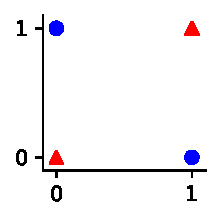
\includegraphics{figures/chapter1/xor_function.pdf}
%   \caption{Graphical representation of the XOR function. This function cannot be separated by a linear classifier.}
%   \label{figure:xor_function}
% \end{figure}
% To circumvent these limitations, \citet{minsky1969perceptrons} considered that \emph{another layer of logic} could be added to the function allowing the classification to be done on another representation (see Figure~\ref{figure:multi_layer_perceptron}).
% Let $\phi_1$ and $\phi_2$ be two linear functions, we could define a \emph{Multi-Layer Perceptron} as follows:
% \begin{equation}
%   f(\xvec) = \rho \circ \phi_2 \circ \rho \circ \phi_1( \xvec )
% \end{equation}
%
%
% One of the first \emph{Multi-Layer Perceptron}, or now more commonly known as \emph{Deep Neural Network}, was introduced by~\citeauthor{ivakhnenko1967cybernetics} in~\citeyear{ivakhnenko1967cybernetics}.
% More precisely, a Neural Neural can be analytically described as a composition of linear functions interlaced with non-linear functions (also called activation functions):
% \begin{equation}
%   f_\Theta(\xvec) = \phi_{\Wmat_p} \circ \rho \circ \phi_{\Wmat_{p-1}} \circ \cdots \circ \phi_{\Wmat_2} \circ \rho \circ \phi_{\Wmat_1}(\xvec)
%   \label{equation:neural_network}
% \end{equation}
% where $p$ corresponds to the \emph{depth} of the network (\ie, the number of layers), the function $\phi_{\Wmat_i}$ is a linear function parameterized by $\Wmat_i$, $\rho$ is a non-linear function and $\Theta \triangleq ( \Wmat_1, \dots, \Wmat_p )$.
% If the weight matrices $\Wmat_i$ are dense, this architecture is called \emph{Fully Connected Neural Network} because all the neurons from the first activation are connected to all the neurons from the second activation.
%
% Therefore, a neural network is a function $f_\Theta:\Rbb^n \rightarrow \Rbb^m$ parameterized by weights and composed of at least two linear functions (layers) and one non-linear function (activation function).
% The input space $n$ corresponds to the dimension of the data and the output space $m$ corresponds to the number of classes the network has to classify. In classical use cases, the dimension of the data is large with respect to the number of classes.
%
%
% %%%%%%%%%%%%%%%%%%%%%%%%%%%%%%%%%%%%%%%%%%%%%%%%%%%%%%%%%%%%%%%%%%%%%%%%%%%%%%%
% \subsection{Introduction to Supervised Learning}
% \label{subsection:ch1-introduction_to_supervised_learning}
% %%%%%%%%%%%%%%%%%%%%%%%%%%%%%%%%%%%%%%%%%%%%%%%%%%%%%%%%%%%%%%%%%%%%%%%%%%%%%%%
%
% This thesis focuses on the concept of \emph{supervised learning} which refers to the notion of learning the parameters of a specific function (neural network) that maps an input to an output based on example input-output pairs.
% For example, an image (input) associated with its content: label (output).
% % The choice of the function used for supervised learning is an active area of research and will be part of the focus of this thesis.


% In the supervised learning framework, the hypothesis space becomes the set of neural networks parameterized by $\Theta$: $\mathcal{H} = \left\{ f_\Theta \ |\ \Theta = ( \Wmat_1, \dots, \Wmat_p ) \right\}$,
% then the learning procedure can be taken over $\Theta$ as follows:
% \begin{equation}
%   \hat{f}^* = \argmin_{\Theta} E(f_\Theta, n) 
% \end{equation}

% Let us consider an input space $\mathcal{X} = \Rbb^d$, an output space $\mathcal{Y} = [k]$ where $k$ is the number of classes and a data distribution $\mathcal{D}$ over $\mathcal{X} \times \mathcal{Y}$.
% In supervised learning, we seek to find a function $h: \mathcal{X} \rightarrow \mathcal{Y}$ that maps the input $\xvec \in \mathcal{X}$ to the output $y \in \mathcal{Y}$ with $h \in \mathcal{H}$ where $h$ is called the \emph{hypothesis} and $\mathcal{H}$ the \emph{hypothesis space}.
% The hypothesis space can take many form but in this work, we will only consider the set of neural networks parameterized by $\Theta$. Therefore, the hypothesis space can be defined as follows:
% \begin{equation}
%   \mathcal{H} = \left\{ f_\Theta \ |\ \Theta = ( \Wmat_1, \dots, \Wmat_p ) \right\}
% \end{equation}
% and the hypothesis is our neural network $f_\Theta \in \mathcal{H}$.
% In order to measure how well the network fits, a \emph{loss function} $L: \mathcal{Y} \times \mathcal{Y} \rightarrow \Rbb^{+}$ is defined.
% The \emph{risk} $R$ associated with the $f_\Theta(\xvec)$ is defined as follows:
% \begin{equation}
%   R(\Theta, \mathcal{D}) \triangleq \Ebb_{(\xvec, y) \sim \mathcal{D}}\  L \left( f_\Theta(\xvec), y \right)
% \end{equation}
% The goal of a \emph{learning algorithm} is to find a network $f_\Theta^* \in \mathcal{H}$ which minimizes the risk $R(\Theta, \mathcal{D})$:
% \begin{equation}
%   f_\Theta^* \triangleq \argmin_{\Theta} R(\Theta, \mathcal{D}) .
% \end{equation}
%
% However, in practice, the joint probability distribution $\mathcal{D}$ is unknown.
% Instead, we have $n$ independent observations of the distribution called the \emph{training set} defined as follows:
% \begin{equation}
%   \mathcal{T} \triangleq \left\{ (\xvec^{(1)}, y^{(1)} ), \dots, ( \xvec^{(n)}, y^{(n)} ) \right\} ,
% \end{equation}
% where $\xvec \in \mathcal{X}$ and $y \in \mathcal{Y}$.
% The risk minimization problem is therefore replaced by the \emph{empirical risk minimization} (ERM) as follows:
% \begin{equation}
%   E(\Theta, \mathcal{T}) \triangleq \frac{1}{|\mathcal{T}|} \sum_{(\xvec, y) \in \mathcal{T}} L\left(f_\Theta(\xvec), y \right) ,
% \end{equation}
% The learning algorithm is adapted to discovers the hypothesis $\hat{f}^*_\Theta$ that minimizes the empirical risk instead of the actual risk.
%
% In recent years, Deep Neural Networks have achieved state-of-the-art performances in a variety of domains such as image recognition~\cite{lecun1998gradient,krizhevsky2012imagenet,he2016deep,tan2019efficientnet}, object detection~\cite{redmon2016you}, natural language processing~\cite{radford2018Language, xxx}, speech recognition~\cite{hinton2012deep, xxx}, etc. 
% However, these performance have been \todo{continue here}
%
% %%%%%%%%%%%%%%%%%%%%%%%%%%%%%%%%%%%%%%%%%%%%%%%%%%%%%%%%%%%%%%%%%%%%%%%%%%%%%%%
% \section{Introducing Structure into Deep Neural Networks}
% \label{section:ch1-introducting_structure_into_deep_neural_networks}
% %%%%%%%%%%%%%%%%%%%%%%%%%%%%%%%%%%%%%%%%%%%%%%%%%%%%%%%%%%%%%%%%%%%%%%%%%%%%%%%
%
% Fully connected neural networks can have a very large number of parameters with respect to the number of data points used in real-world datasets.
% For example, with the MNIST dataset~\cite{lecun1998gradient} which consist of $5 \times 10^4$ images of handwritten digits from 0 to 9, a two-layer fully connected neural network will have more than $6 \times 10^5$ parameters.
% Training such a large network has a number of significant drawbacks: they are hard to train, subject to overfitting and are computationally expensive.
% To overcome these limitations, \citet{vapnik1992principles} have proposed to replace the empirical risk minimization principle by \emph{structural risk minimization} (SRM) which consists of implementing ERM with the addition of a structure on the hypothesis space.
% \todo{ajouter explication intuitive pourquoi ajouter de la structure permet de résoudre les problèmes}
% Adding a structure on the hypothesis space can be done using two methods: constraining the architecture of the network or constraining the learning procedure by adding a regularization term. 
% Hereafter, we present in more detail the two approaches.  
%


% \paragraph{Structural Risk Minimization} (SRM).
% The ERM principle assumes that the function $\hat{h}^*$ minimizing $E(h, n)$ leads to the risk $R(\hat{h}^*)$ being close to the minimum.
% This assumption mean that as the \emph{size} of the training set increase the minimization becomes more accurate. More formally, the ERM principle assumes that $R(\hat{h}^*)$ converge to its minimum value on the set $h \in \mathcal{H}$ when $n \rightarrow \infty$.  
% \citet{Vapnik1991TheNA} have shown that this equivalent to say that the empirical risk $E(h, n)$ \emph{converge uniformly} to the actual risk $R(h)$ over $h \in \mathcal{H}$ where the \emph{uniform convergence} is defined as follows:
% \begin{equation}
%   \Pbb \left[ \sup_{h \in \mathcal{H}} \left| R(h) - E(h, n) \right| < \epsilon \right] \rightarrow 0 \quad \text{ when } \quad n \rightarrow \infty, \quad \forall \epsilon > 0 
% \end{equation}

% %%%%%%%%%%%%%%%%%%%%%%%%%%%%%%%%%%%%%%%%%%%%%%%%%%%%%%%%%%%%%%%%%%%%%%%%%%%%%%%
% \subsection{Structure Given by the Architecture of the Neural Network}
% \label{subsection:ch1-introducing_structured_into_the_architecture_of_neural_networks}
% %%%%%%%%%%%%%%%%%%%%%%%%%%%%%%%%%%%%%%%%%%%%%%%%%%%%%%%%%%%%%%%%%%%%%%%%%%%%%%%
%
% \begin{figure}[htb]
%   \centering
%   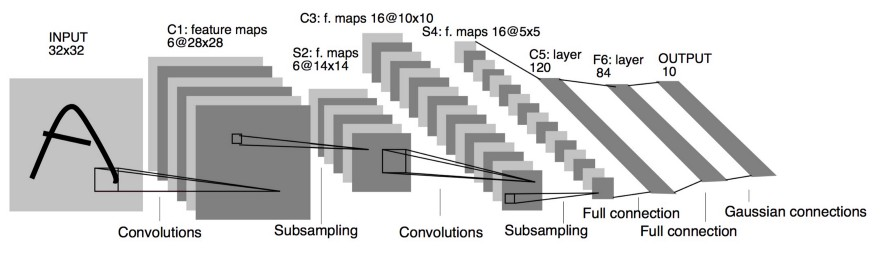
\includegraphics[scale=0.4]{figures/chapter1/lenet.jpg}
%   \caption{Graphical representation of the LeNet architecture proposed by \citet{lecun1998gradient}}
%   \label{figure:lenet_network}
% \end{figure}
%
% An example of neural networks with a specific architecture are \emph{Convolutional Neural Networks} (CNN)~\cite{lecun1998gradient,krizhevsky2012imagenet,he2016deep,tan2019efficientnet} which consists of neural networks with specific structured linear transform. 
% This transform used in convolutional layers is the discrete convolution which consists of a kernel sliding over the image and acting as a filter.
% % A perfect example of such efficient linear operation is the discrete convolution which consists of a kernel sliding over the image and acting as a filter.
% Let $\avec$ and $\bvec$ be two vectors, the discrete convolution between the signals $\avec$ and $\bvec$ denoted $a \ast b$ is given by: 
% \begin{equation}
%   (\avec \ast \bvec)_i \triangleq \sum_{j = -m}^m \avec_j \cdot \bvec_{i - j}
% \end{equation}
% The convolution operation has translation invariance characteristics \cite{zhang1990parallel} which is perfectly suited for image classification (objects can be at different positions in images).  
% \citet{lecun1998gradient} was one of the first to successfully train a convolutional neural network, achieving state-of-the-art performance on the MNIST dataset.
% Convolution neural networks achieve a good performance for two main reasons:
% first, CNNs are similar to the connectivity pattern of neurons in the visual cortex of the human brain. 
% Secondly, CNNs are very efficient due to the sharing of parameters. 
% While a classical linear operation with dense matrix has $n \times n$ parameters, a convolution only has $k \times k$ parameters where $k$ is the kernel size and is usually small (\eg 3 or 5 for classical convolution layers use in neural networks).
% This weight sharing reduces the number of weights with respect to the fully connected neural network. The LeNet architecture (see Figure~\ref{figure:lenet_network}) has only $6 \times 10^4$ parameters.  
%
% Although, convolutional neural networks have demonstrated good results on a specific type of applications (in particular image processing). 
% It remains unclear whether other types of structure can be beneficial to other types of applications.
% Can we use other types of structure for neural networks?  
% Does the reduction of parameters reduce the performance of the network?
%



% %%%%%%%%%%%%%%%%%%%%%%%%%%%%%%%%%%%%%%%%%%%%%%%%%%%%%%%%%%%%%%%%%%%%%%%%%%%%%%%
% \subsection{Structure Given by the Learning Procedure}
% \label{subsection:ch1-introducing_structured_into_the_learning_procedure}
% %%%%%%%%%%%%%%%%%%%%%%%%%%%%%%%%%%%%%%%%%%%%%%%%%%%%%%%%%%%%%%%%%%%%%%%%%%%%%%%


% Instead of constraining the architecture of the network, we can constrain the learning procedure in order to reduce the search space.
% Consider the following hypothesis space $\mathcal{H} = \left\{ f_\Theta \ |\ \Theta = ( \Wmat_1, \cdots, \Wmat_p ) \right\}$ which define the set of neural networks with fixed architecture.
% We can introduce a structure in the hypothesis space by setting:
% \begin{equation}
%   \mathcal{H} = \left\{ f_\Theta \ |\ \Theta = ( \Wmat_1, \cdots, \Wmat_p ) \ |\ R(\Theta) \right\} 
% \end{equation}
% where $R(\Theta)$ is a constrain on $\Theta$ called a regularizer.

% Instead of constraining the architecture of the network, we can impose a penalty on the \emph{complexity} of $f_\Theta$.
% The notion of \emph{complexity} can, for example, includes restrictions for smoothness and/or bounds on the vector space norm.
% For example, let us consider the following constrained hypothesis space:
% \begin{equation}
%   \mathcal{H}_\epsilon = \left\{ f_\Theta \ |\ \Theta = ( \Wmat_1, \cdots, \Wmat_p ) \ |\ R(\Theta) \leq \epsilon \right\} 
% \end{equation}
% where $R(\Theta)$ is a constrain on the weights called a regularizer.
%
% One of the most common form of regularization \cite{tikhonov_arsenin_1977, krogh1992simple} consists of adjusting the weights during the learning procedure under the constraint to keep the magnitude of the weights small, in this case, the regularizer $R(\Theta)$ can be defined as follows:
% \begin{equation}
%   R(\Theta) = \sum_{i=1}^p \norm{\Wmat_i}_\mathrm{F} 
% \end{equation}
%
%
%
% This regularization has been introduced by~\citet{tikhonov_arsenin_1977} and is commonly known as \emph{weight decay}.
% \todo{we need to cite the paper NIPS krogh1992simple}
% \cite{krogh1992simple}
% With this constraint, the hypothesis space can be defined as follows:
% \begin{equation}
%   \mathcal{H_\epsilon} = \left\{ f_\Theta \ |\ \Theta = (\Wmat_1, \cdots, \Wmat_p) \ | \ \norm{\Wmat_i}_\mathrm{F} \leq \epsilon \right\} 
% \end{equation}
% For a convex loss function, the minimization of the empirical risk within the set $\mathcal{H}_\epsilon$ can be achieved with the minimization of
% \begin{equation}
%   E(f_\Theta, n, \lambda) = \frac{1}{n} \sum_{i = 1}^{n} L\left(f_\Theta(\xvec^{(i)}), y^{(i)} \right) + \lambda \sum_{i = 1}^{p} \norm{\Wmat_i}_\mathrm{F}
% \end{equation}
% \todo{we need to cite kuhn2014nonlinear,karush1939minima}
% \cite{kuhn2014nonlinear,karush1939minima}
% where $\lambda$ is a Lagrange multiplier.
%
% Defining a regularization strategy is still an open problem in supervised learning. Recent works have proposed different forms of regularization.  
%









